% Figure 1: one task, from the request to the answer, as a sequence of
% messages between the child's card, the chat's model, the service and the
% parent's Google Drive, on the path where the task is accepted. The paper's
% preamble defines \System and loads TikZ; arrows use only the tips TikZ has
% without a library. Each party's column is set once, below, and every arrow
% stands on those columns.
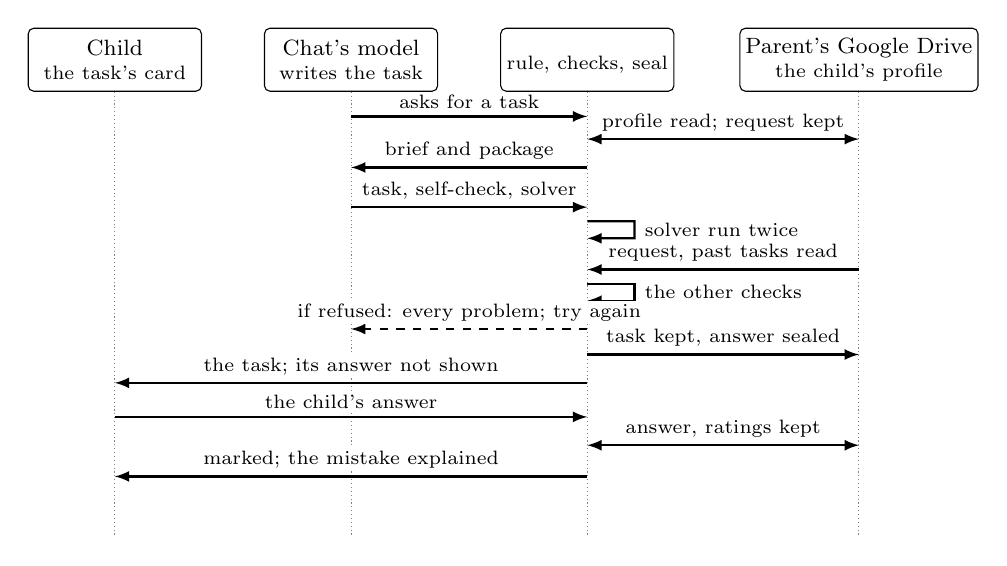
\begin{tikzpicture}[
  y=0.72cm,
  font=\footnotesize,
  >=latex,
  party/.style={draw, rounded corners=2pt, align=center, minimum width=22mm, minimum height=8mm, inner sep=2pt},
  life/.style={densely dotted, gray},
  msg/.style={->, thick},
  back/.style={->, thick, dashed},
  trip/.style={<->, thick},
  note/.style={font=\scriptsize, align=center, fill=white, inner sep=1pt, above=1.5pt},
  aside/.style={font=\scriptsize, align=left, right},
]
  \def\xCard{0}\def\xModel{3.0}\def\xService{6.0}\def\xDrive{9.45}

  % The four parties, left to right, and their lifelines.
  \node[party] (card)    at (\xCard,0)    {Child\\[-1pt]{\scriptsize the task's card}};
  \node[party] (model)   at (\xModel,0)   {Chat's model\\[-1pt]{\scriptsize writes the task}};
  \node[party] (service) at (\xService,0) {\System\\[-1pt]{\scriptsize rule, checks, seal}};
  \node[party] (drive)   at (\xDrive,0)   {Parent's Google Drive\\[-1pt]{\scriptsize the child's profile}};
  \foreach \p in {card, model, service, drive}
    \draw[life] (\p.south) -- ++(0,-7.85);

  % The request: the rule reads the profile, keeps the request in it and
  % writes the brief.
  \draw[msg]  (\xModel,-1.0)    -- node[note] {asks for a task} (\xService,-1.0);
  \draw[trip] (\xService,-1.4)  -- node[note] {profile read; request kept} (\xDrive,-1.4);
  \draw[msg]  (\xService,-1.9)  -- node[note] {brief and package} (\xModel,-1.9);

  % The task: its solver runs before the profile is read; the other checks
  % need the request and the child's past tasks; a refused task goes back.
  \draw[msg]  (\xModel,-2.6)    -- node[note] {task, self-check, solver} (\xService,-2.6);
  \draw[msg]  (\xService,-2.85) -- ++(0.6,0) -- node[aside] {solver run twice} ++(0,-0.3) -- (\xService,-3.15);
  \draw[msg]  (\xDrive,-3.7)    -- node[note] {request, past tasks read} (\xService,-3.7);
  \draw[msg]  (\xService,-3.95) -- ++(0.6,0) -- node[aside] {the other checks} ++(0,-0.3) -- (\xService,-4.25);
  \draw[back] (\xService,-4.75) -- node[note] {if refused: every problem; try again} (\xModel,-4.75);
  \draw[msg]  (\xService,-5.2)  -- node[note] {task kept, answer sealed} (\xDrive,-5.2);
  \draw[msg]  (\xService,-5.7)  -- node[note] {the task; its answer not shown} (\xCard,-5.7);

  % The answer: unsealed, marked and explained; the ratings move.
  \draw[msg]  (\xCard,-6.3)     -- node[note] {the child's answer} (\xService,-6.3);
  \draw[trip] (\xService,-6.8)  -- node[note] {answer, ratings kept} (\xDrive,-6.8);
  \draw[msg]  (\xService,-7.35) -- node[note] {marked; the mistake explained} (\xCard,-7.35);
\end{tikzpicture}
